We used adaptive dynamics theory to study the conditions favorable to parapatric adaptive speciation in a sexual, diploid species spread across two patches. 

% Divergent selection determines whether branching occurs in full sympatry

\paragraph{Divergent selection determines whether branching occurs in full sympatry} The strength of divergent selection is an important parameter in determining whether branching will occur. Whether selection is needed to trigger branching depends on environmental heterogeneity. When the landscape is homogeneous (habitat symmetry  is $1$), a minimal amount of selection is needed for branching to occur (Fig. \ref{fig:map_branching_points}). This minimum amount is a selection coefficient value of $s = 0.5$, which is the point at which the reproductive success function $W$ (proportional to the sum of the two attack rate functions in Fig. \ref{fig:attack_rates} in a homogeneous environment) goes from being unimodal to being bimodal, thus producing two peaks in the adaptive landcape. For $s > 0.5$, specialists i.e. individuals with trait values closer to $\pm 1$, have a higher payoff than generalists i.e. individuals with trait values closer to zero. Although a two-peaked fitness landscape imposed by the resources would in itself favor the splitting of a population only if this population is sitting at the bottom of the valley between the two hills, branching can occur even when starting with a specialist population (e.g. with initial trait value $x = -1$ in Fig. \ref{fig:map_branching_points}) because of disruptive frequency-dependent selection arising as a result of competition. This case is analogous to the classical sympatric speciation scenario.\\

% Environmental heterogeneity promotes divergence without divergent selection

\paragraph{Environmental heterogeneity promotes divergence without divergent selection} On the contrary, when habitat heterogeneity increases, divergent selection may be less, or not at all, needed for branching. This is because as habitat asymmetry increases, one resource becomes more abundant and more advantageous to exploit in one of the two habitats, while the other resource becomes more advantageous in the other habitat. This creates conditions for directional, and eventually stabilizing, selection and local adaptation within each habitat, albeit in opposite directions between the two habitats. This scenario is such that at high levels of habitat asymmetry, the payoff obtained by exploiting the least abundant resource is so low that the fitness landscape is almost entirely determined by the most abundant resource. Selection will push towards that peak, even if the slopes are very shallow, just because there is no other peak, and the opposite will happen in the other habitat, resulting in branching across habitats even under very weak selection (Fig. \ref{fig:map_branching_points}).\\

% Branching is prevented by too strong divergent selection

\paragraph{Branching is prevented by too strong divergent selection} Too strong divergent selection can inhibit branching (Fig. \ref{fig:map_branching_points}). In our two-patch model, the monomorphic population branches by first evolving towards the point $x = 0$ and then splitting, even though the two habitats may select for different optima (this is because the habitats are mirror-images of each other). Above a certain value of the selection coefficient, this point becomes an unattainable tipping point, i.e. an evolutionary repellor under which a population is pushed to evolve towards more negative values and above which it evolves more positive values. The population eventually stabilizes at either specialist strategy, depending on the starting conditions. This upper limit decreases with increasing habitat asymmetry (Fig. \ref{fig:map_branching_points}). This is because selection against intermediate forms becomes so strong that a monomorphic population can no longer evolve to the generalist branching point in the first place; it becomes convergence unstable (Fig. \ref{fig:pairwise_invasibility}). The population will evolve towards one of the two specialists, even if it starts at the tipping point because the two specialists cannot coexist (am I correct, Sander?). The upper limit of selection strength allowing branching goes down as asymmetry rises (Fig. \ref{fig:map_branching_points}). This is because in a heterogeneous environment, the lower availability of one of the two resources imposes extra within-patch directional selection and thus reinforces selection against generalists, even at levels of divergent selection that would allow for branching in a homogeneous case.\\

% Whether branching occurs depends on the starting conditions

\paragraph{Whether branching occurs depends on the starting conditions} An ecological generalist is more likely to undergo branching than a specialist. The upper limit of selection strength that allows for branching is lower when a population is initialized with a trait value of $-1$, that is, a specialist of the first resource, than what is theoretically feasible (Fig. \ref{fig:map_branching_points}). This is because as selection increases, there comes a point at which the specialist strategy becomes a stable strategy and an evolutionary attractor. At this point there are multiple attractors, and convergence towards either strategy depends on the starting trait value; where selection is strong enough that an initial specialist will experience stabilizing selection to remain at its original fitness peak, while an initial trait value closer to the generalist strategy will evolve towards the generalist type and branch. This can be seen in Figure \ref{fig:pairwise_invasibility}, where the generalist strategy ($x = 0$) is still a branching point at $s = 2$, making branching in theory possible, but where each specialist ($x = \pm 1$) is an evolutionarily stable strategy. In these conditions, phenotype space is separated into three basins of attraction, each leading to one of the three convergent strategies, and whether branching will occur depends on the starting conditions. As selection intensifies, the basin of attraction of the two specialist strategies expands, while the one of the generalist shrinks. Branching then becomes more and more restricted to populations starting closer to zero, up to the point where the generalist becomes a repellor (e.g. at $s = 2.5$ in Fig. \ref{fig:pairwise_invasibility}) and branching is no longer possible.\\

% Reduced gene flow facilitates local adaptation

\paragraph{Reduced gene flow facilitates local adaptation} Geographic barriers to gene flow are a well-known facilitator of speciation. Here, a reduction in dispersal rate $m$ (analogous to a stronger geographical barrier) enhances divergence because it facilitates local adaptation. By making the two habitats more independent of each other in their dynamics, reduced gene flow enhances the disruptive effect of environmental heterogeneity mentioned above. Increasing gene flow, on the other hand, brings the landscape closer to a homogeneous scenario, where e.g. a minimum amount of divergent selection is needed to trigger branching (Fig. \ref{fig:map_branching_points}).\\

% Sexual selection counteracts divergent adaptation

\paragraph{Sexual selection counteracts divergent adaptation} We showed in Equation \ref{eq:curvature_final} that sexual selection increases the evolutionary stability of the singular strategy. This is visible in Figure \ref{fig:map_branching_points} where increasing values of the sexual selection coefficient $\alpha$ reduce the range of conditions for branching, by turning branching points into evolutionarily stable strategies. This stabilizing effect of sexual selection is particularly strong in a homogeneous environment, where branching becomes drastically more restricted to higher divergent ecological selection values as sexual selection increases. This effect is mediated by environmental heterogeneity, as branching is recovered under stronger sexual selection when habitat asymmetry increases or gene flow decreases (Fig. \ref{fig:map_branching_points}).\\

% Selection and environmental heterogeneity promote divergence between patches

\paragraph{Selection and environmental heterogeneity promote divergence between patches} Studying the adaptive dynamics in the absence of dispersal ($m = 0$) in the two patches separately allows to disentangle the effects of divergent local adaptation across patches and competition within patches as a cause for branching. Divergence in equilibrium trait values between the two habitats is shown in Figure \ref{fig:map_divergence} across parameter space. As expected, increasing habitat asymmetry promotes divergence across patches because of differences in resource availability. Stronger divergent selection reinforces this effect. Although there seems not to be any upper limit to the level of divergent selection that allows allopatric phenotypic divergence when the two populations are initially generalists ($x = 0$, Fig. \ref{fig:map_divergence}A), there is a hard limit when the populations are initially identical specialists ($x = -1$, Fig. \ref{fig:map_divergence}B), above which the populations remain identical. If selection is too strong, a population starting at $-1$ will stay at $-1$ even in a very asymmetric environment, because the alternative specialist strategy is too far away in trait space and cannot be achieved by small substitutions.\\

% Branching within patches occurs if selection is strong enough, but not too strong, and if environmental heterogeneity is not too high

\paragraph{Branching within patches occurs if selection is strong enough, but not too strong, and if environmental heterogeneity is not too high} In addition, as the two populations diverge in allopatry, they may also each reach a branching point and split into two sympatric morphs independently because of frequency-dependent selection induced by competition (yellow area in Fig. \ref{fig:map_divergence}). With our settings, whenever within-patch branching occurs in one habitat, it occurs in the other as well, because habitats are mirror images of each other. The branching point that is reached through evolution may not be the same in both habitats, and their divergence also increases with habitat asymmetry (Fig. \ref{fig:map_divergence}). Our results show that branching in sympatry occurs only provided that divergent selection is strong enough ($s > 0.5$) and that habitats are not too asymmetric. If selection is too low, a generalist type is favored over either specialist (see Fig. \ref{fig:pairwise_invasibility}, $s = 0.01$). If habitats are too asymmetric, local adaptation evolves instead of branching, and divergence is in allopatry. Too strong selection would also reinforce the effect of habitat asymmetry and promote allopatric divergence rather than sympatric branching; as Figure \ref{fig:map_divergence}A shows that the upper limit of selection allowing for branching increases as the environment becomes more homogeneous. The starting conditions also affect whether sympatric branching can occur; as divergent selection increases, an initial specialist will be trapped quicker at its starting point than a generalist that is located closer to the branching point. Note that in this case, the branching point within a patch is not located at zero when the habitats are not fully symmetric, but is still exactly opposite to the branching point in the other patch.

\begin{figure}
    \centering
    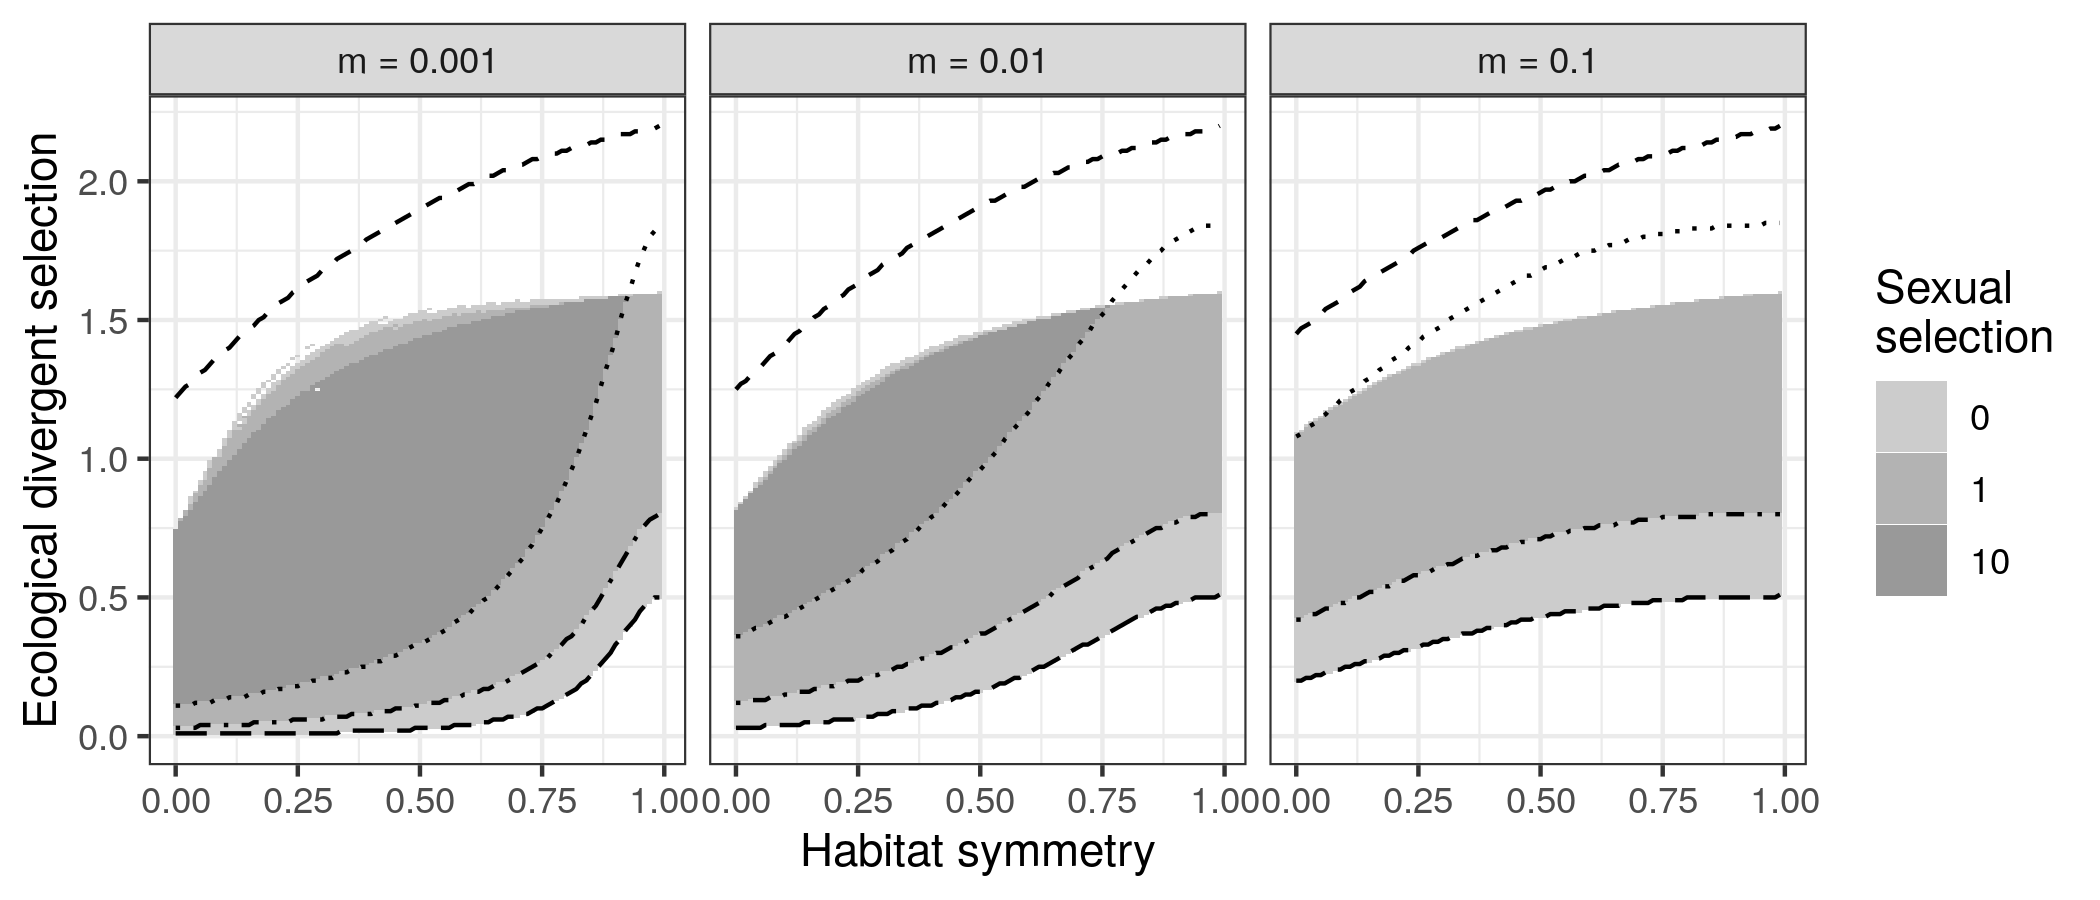
\includegraphics[width=\textwidth]{figures/map_branching_points}
    \caption{Branching throughout parameter space for three values of the dispersal rate $m$. Sexual selection increases the stability of evolutionary equilibria and therefore turns branching points into stable strategies. Shades of grey indicate the highest tested level $\alpha$ of sexual selection at which branching still occurs when a population is initially a specialist of the first resource ($x = -1$). Dashed lines expand the borders of the grey areas to show the full extent of where branching can theoretically occur, irrespective of the starting trait value. Parameters, $a = 400$, $b = 100$, $d = 0.2$, $\alpha = 0$. The results do not depend on the value of $\alpha$ here (really?).}
    \label{fig:map_branching_points}
\end{figure}

\begin{figure}
    \centering
    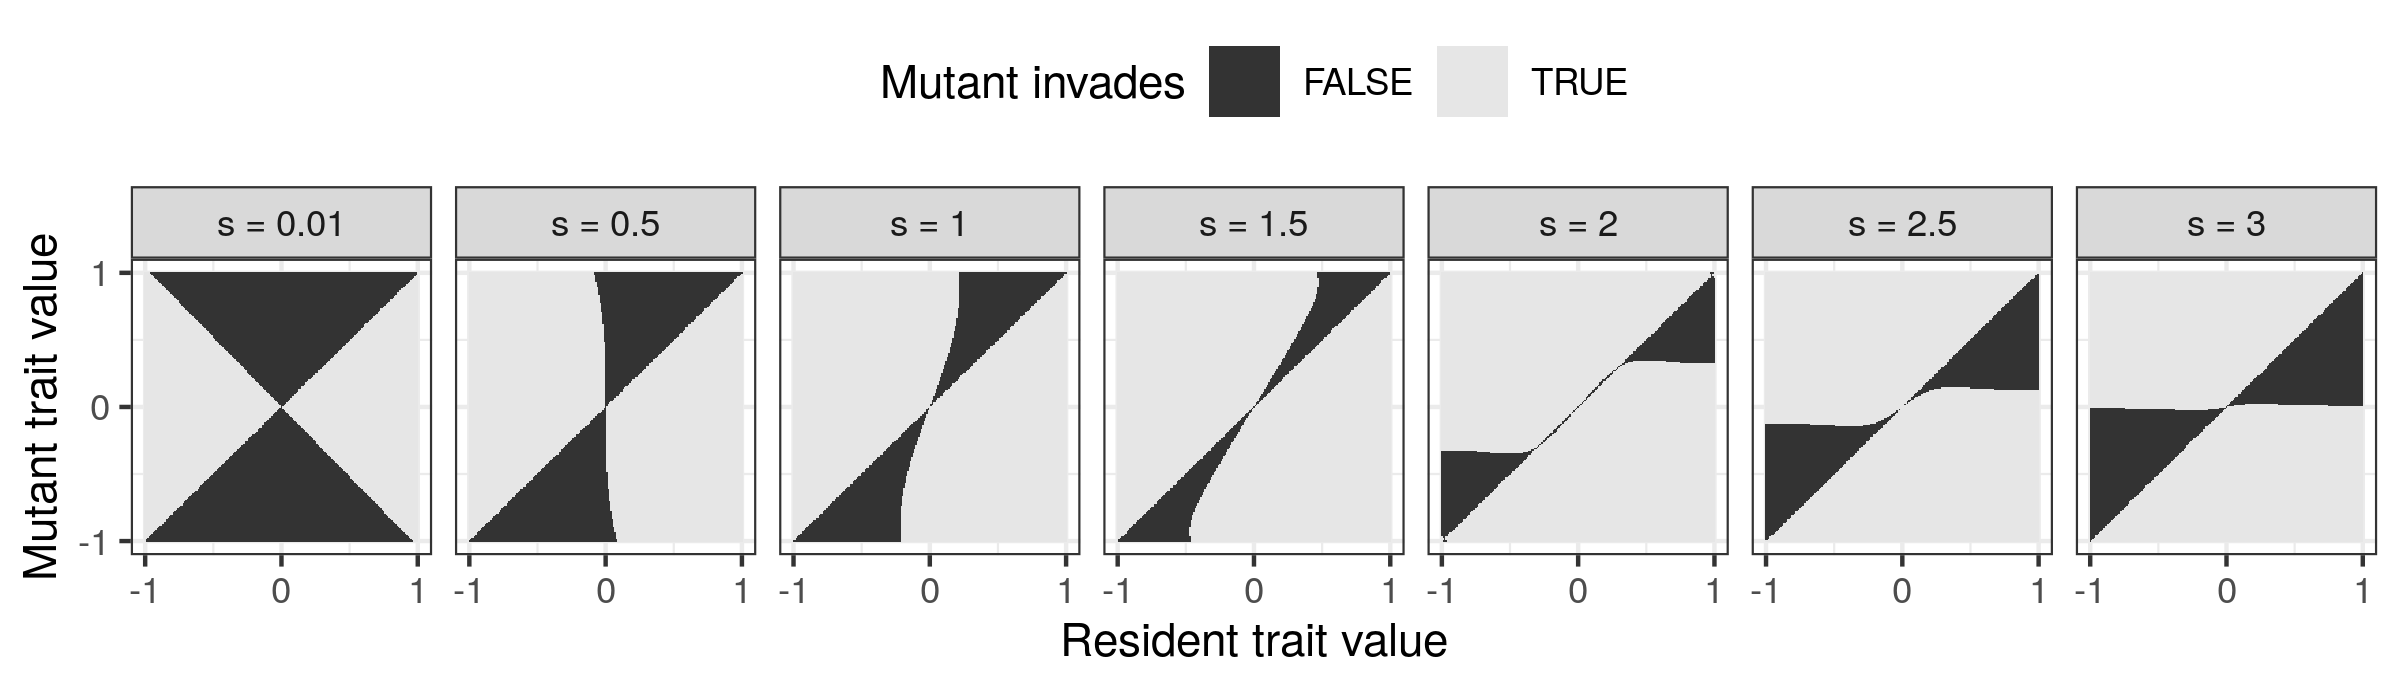
\includegraphics[width=\textwidth]{figures/pairwise_invasibility_plots}
    \caption{Pairwise invasibility plots showing how the singular trait value $x = 0$ changes from being an evolutionarily stable strategy to being a repellor tipping point through being a branching point, along a gradient of divergent selection coefficient values $s$. Parameter values, $a = 400$, $b = 100$, $h = 1$, $d = 0.2$, $m = 0.01$, $\alpha = 0$.}
    \label{fig:pairwise_invasibility}
\end{figure}

\begin{figure}
    \centering
    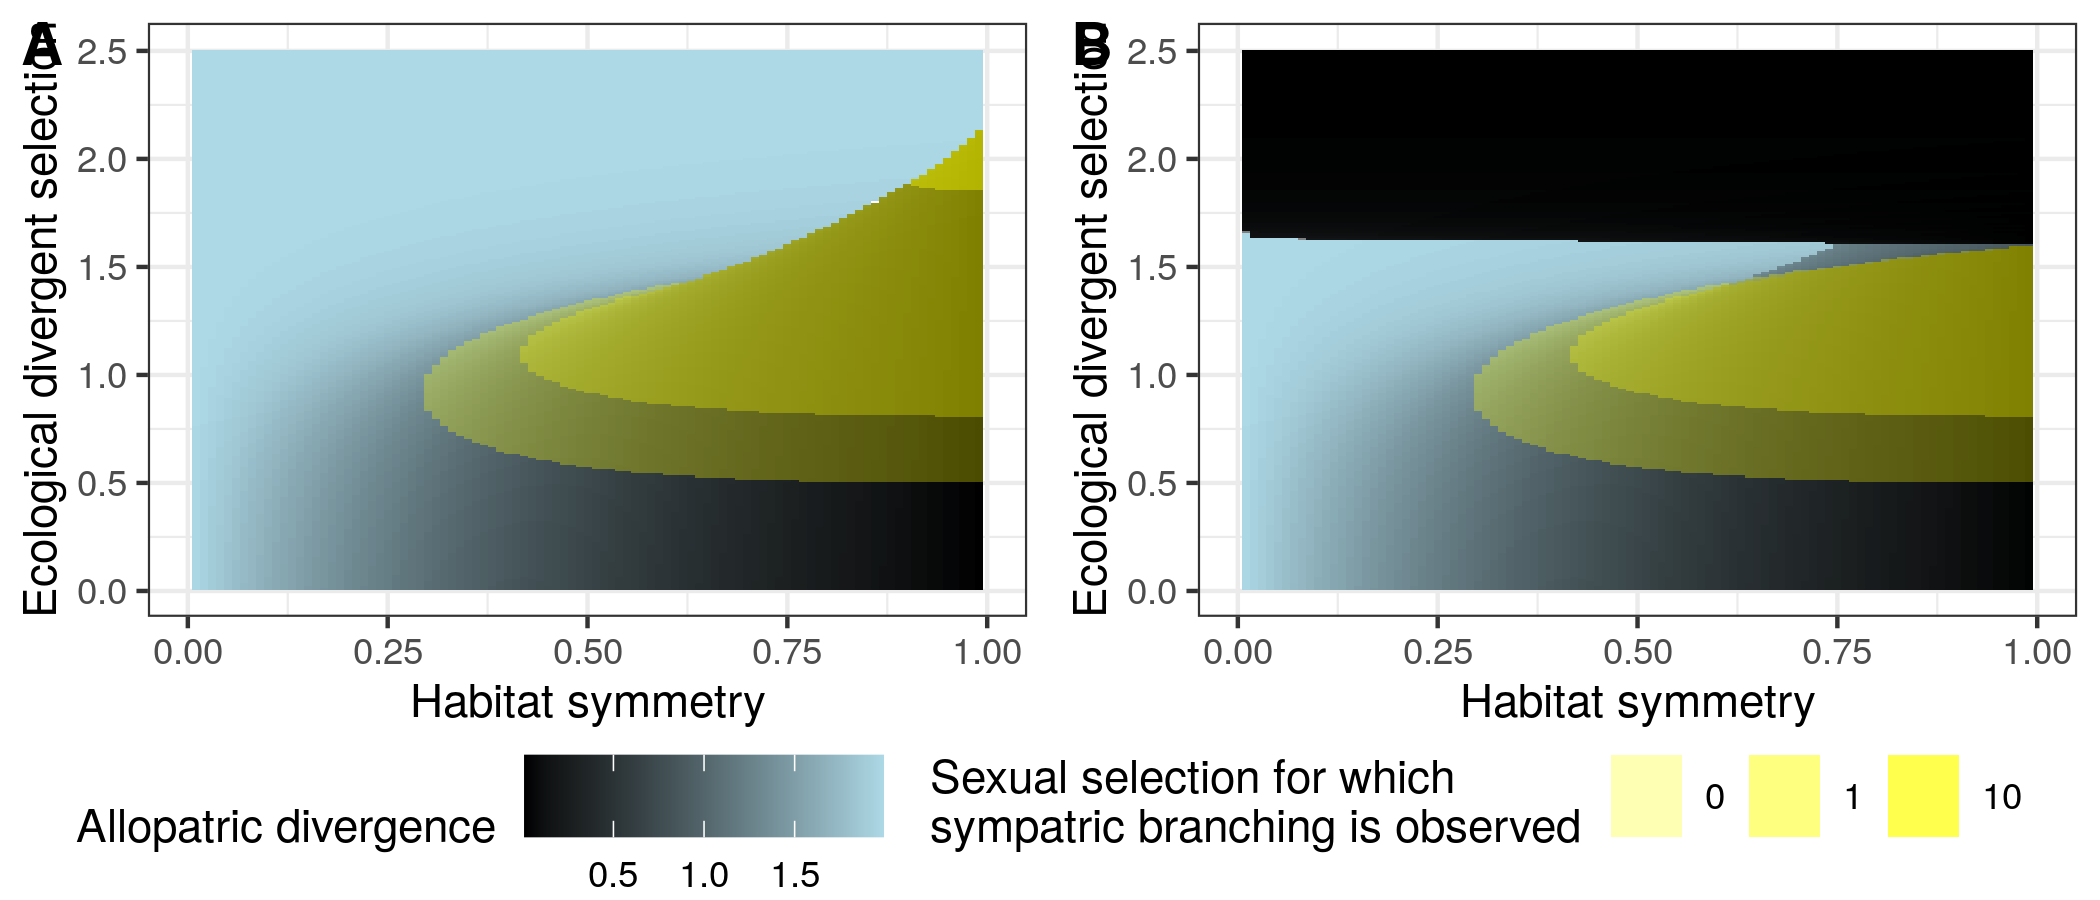
\includegraphics[width=\textwidth]{figures/divergence_across_patches}
     \label{fig:map_divergence}
\end{figure}